\documentclass{article}
\usepackage{graphicx}
\usepackage{float}
\usepackage{fancyhdr}
\usepackage{lastpage}

\pagestyle{fancyplain}

\lhead{Group Project 14 - Design specification/1.0/(For review)}
\lfoot{Aberystwyth University / Computer Science}
\rhead{ }
\rfoot{Page \thepage\ of \pageref{LastPage}}
\cfoot{ }


\begin{document}

\title{Group Project 14 - Design specification}
\author{Lars Hudson Lunde}
\date{\today\\Version 1.0}
\maketitle

\makebox[\textwidth]{Config Ref: SE.D.DESIGN.01} \par
\makebox[\textwidth]{Status: For review} \par


\clearpage
\tableofcontents
\clearpage

\section{Introduction}
\textbf{Author: Lars H Lunde}
\bigskip

This document is the project plan for the Walking Tour Creator

\subsection{Purpose of Document}
The purpose of this document is to describe the design of
the project as concluded by the group from the specification.

\subsection{Scope}
This document shows the overview of the system, the use-cases and 
user interface for both app and web side, the time schedule for the project
and the an analysis of the risks of the project not completing.

\subsection{Objective}
The main objective of this document is to show the design of the system
being made, and when how and with what tools it will be made, and at what times
the different components need to be done. Also making clear what can be done
for users and administrators from both phone and web side.


\section{Overview of proposed system}
\textbf{Author: James Mellor}
\bigskip

\subsection{Project Overview}
Our app that we are having to produce is going to be an android based app.
Are app is going to be a walking app that will help people make their own 
walks and to be able to edit and save them to use again a later day.
\bigskip

Platforms to be used and Architecture for the app:
\bigskip

\subsubsection{Android}
The assignment stated that we have to make an app for android 
phones so thats the platform we will be using.

\subsubsection{PHP}
We will be using PHP for the website and for the phone to communicate 
to the website (database). I think we will find it easier to use then 
javascript and it will be a good opportunity to get better at writing 
in that language. 

\subsubsection{JAVA}
Java is what we will be using to program the app. We just need to
decide what we will use to write it in, their is a choose between
eclipse with the plug in or android studio. I can imagine we will 
be using android studio.

\subsubsection{MySQL}
MySQL is what we will be using to make the database to be able 
to store the walks that have been created. 

\subsection{High Level Architecture}
\subsubsection{Map API}
The map will be a big part of are app because we will need to display the
routes and be able to let people see where there going and make their own
route. We will be using the google maps api for this with the ability to 
be able to zoom in and out, here there will be options to save route and 
add location. The map will have markers on it to show where to go or how 
the map is being plotted.

\subsubsection{App UI}
The Menu / UI, first we will have the main page where from here you will 
be able to click on the button create new route to be able to start mapping 
the path while you are walking, right underneath this button their will be 
2 more preferences and exit. All together there will be up to 4 menus to 
this app: main page, naming of the walk, route map editor and the adding location. 

\subsubsection{Internet Usage}
The app will only need to use the wifi or 3G/4G to be able to improve 
the tracking capability of the app and to be able to upload the finished walks onto the website.

\subsubsection{Target Users}
Are target users are people that enjoy going on walks and would like to start marking 
out their walks and to be able to save them so they can look back at them and do the walk a later day. 

\clearpage
\section{Use-cases}
\textbf{Author: Rob Bolton}
\bigskip

The use cases for our application will be split into two cases.\newline
These are the "App" and the "Server".\newline
The App use case describes all interaction with the application itself and, as such, 
only contains interaction with the mobile user. The server is not listed as interacting 
with the app here as interaction between the app and the server is functionally one-way 
(the app pushes walks to the server, but cannot retrieve or view walks).\newline
The Server use case describes all interaction with the server, which includes the web 
user, app, and administrative user. 

\subsection{App}
\begin{figure}[H]
    \makebox[\linewidth]{
        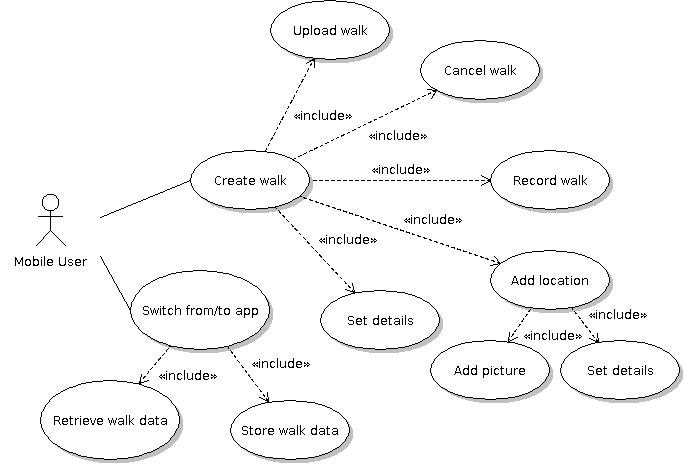
\includegraphics[width=1\linewidth]{AppUseCase}
    }
\end{figure}

\clearpage
The app's use cases include: 

\subsubsection{Create Walk(FR1)}
Here the user starts to create a walk. Once this interaction is started 
(by pressing the button in the app's main menu), and a valid walk name is provided, 
the user's location is tracked and periodically added to the on-going walk's list of GPS points.\newline
As a part of this case the user may choose to: 

\begin{itemize}
\item Add location: This will allow the user to add the current location to the walk as a point of interest. (FR3)
		\begin{itemize}
		\item Take picture: The user can take a picture to add to this location. (FR4)
		\item Set details: The user can set the location's details (name, description).
		\end{itemize}
\item Set details: The user can set the walk's details (title, short decription(<100 characters), long description(<1000 characters). (FR2)
\item Cancel walk: The user may choose at any point to cancel their walk. This will stop recording their position and drop all current data of the on-going walk. (FR5)
\end{itemize}

\subsubsection{Upload Walk (FR6)}
This is used at the end of the "create walk" case in order to upload the walk to the server.

\subsubsection{Switch to/from app}
Whenever the user switches from the WTC app to another app, it will store the current walk's data. When they switch back it will retrieve the previously stored data. (FR7)

\subsection{Server}
\begin{figure}[H]
    \makebox[\linewidth]{
        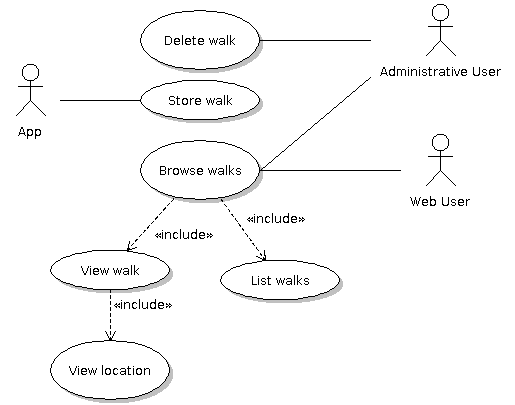
\includegraphics[width=1\linewidth]{ServerUseCase}
    }
\end{figure}

The server's use cases include several actors. \newline
The "App" actor is an instance of the WTC app on a client's phone and can upload walks. \newline
The "Web User" is a client accessing the WTC website in a web browser. 
They may view a list of walks, select one, and view its details.\newline
The "Administrative User" is a user with the power to delete walks as well as view them.\newline
\bigskip

The server's use cases include: 

\subsubsection{Store walk}
A walk recieved from a client using the WTC app can be stored in the database of walks. If a walk with the same name exists then it is refused. (FR9)

\subsubsection{Delete walk}
This use case allows for administrative users to delete any walks which they feel do not belong in the database.
This would include any corrupted/broken walks and walks which contain obscene or offensive content. 
 
\subsubsection{Browse walks}
This use case provides html pages to users which contains a list of all the walks in the database. The cases in this case are: 

\begin{itemize}
\item List walks: This provides a list of all the stored walks.
\item View walk: This will allow the user to view a specific walk, including its name, short and long descriptions, and its points of interest. (FR8)
		\begin{itemize}
		\item View location: This will allow a user to look at a specific point of interest. This includes its name, description, location, and any picture it has.
		\end{itemize}
\end{itemize}

\section{User interface design}
\textbf{Authors: Jake Maguire and Michael Oddie}

\subsection{Android Application UI Design}
This section of the documentation will give an idea for how the UI of both the Android application and the web application
will look like and also the flow of the program from screen to screen. These designs are not final due to technical
restraints we may face later on in development but they will give a feel for the sort of layout and feel we are working towards.

\subsubsection{Main Menu (FR1)}
\bigskip
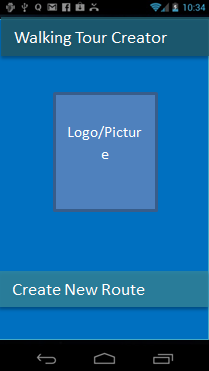
\includegraphics{PhoneUI1}
\bigskip

The first screen that the user is presented with is the main menu. This screen has one main option for the user to select.
The user can create a new route which allows them to progress into the application and start recording their routes.
There will also be some sort of logo or picture above these options.

\subsubsection{Create New Route (FR2)}
\bigskip
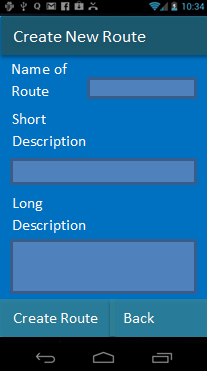
\includegraphics{PhoneUI2}
\bigskip

On the Create New Route screen the user is able to set up a new route for them to record.
They will be presented with a field to enter the name of the route, a short description
of the route and a longer description. The short description will be restricted to up to 
100 characters while the long description is up to 1000 characters. The user will be 
required to fill in all of the fields, as per the functional requirements. 

\bigskip
There will be two buttons at the bottom which allow the route to be created or to go back to the previous page. 

\subsubsection{Create Route (FR1, FR5, FR6)}
\bigskip
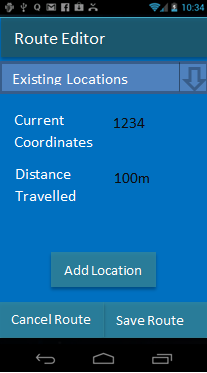
\includegraphics{PhoneUI3}
\bigskip

When the route has been created the user will be presented with their current coordinates which will update in real 
time as the user moves around, their current distance travelled from the starting location, along with options to 
add a location and save the current route.
\bigskip
The existing locations drop down will allow the editing of locations that have already been added, 
letting the user change the name, coordinates and description of a previous location.
\bigskip
Adding a location will save the current position and move to the next screen where they can specify information about that location.
Once the user has finished recording and has added their locations, the user can press the save location button at the bottom of the 
screen to send this data to the server where it can be read by the web application. They can also cancel the walk if they do not require it after recording.

\subsubsection{Adding Location (FR3, FR4, FR9)}
\bigskip
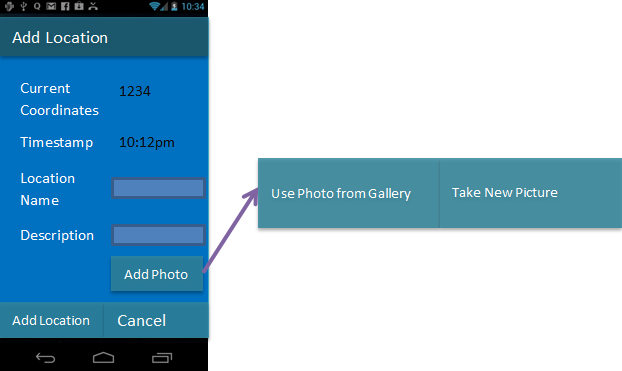
\includegraphics{PhoneUI4}
\bigskip

When adding the location the user is required to enter some information along with some already given to you.
The user�s current coordinates are displayed along with the current time the location was added.
The user then enters the name of the location and a short description.
There is also an option to add a photo where a photo can be taken using the camera option or use a photo already in the gallery.

\subsection{Web Application Design}
\subsubsection{HomePage}
\index{User interface design!Web Application Design!HomePage}
\begin{figure}[H]
    \makebox[\linewidth]{
        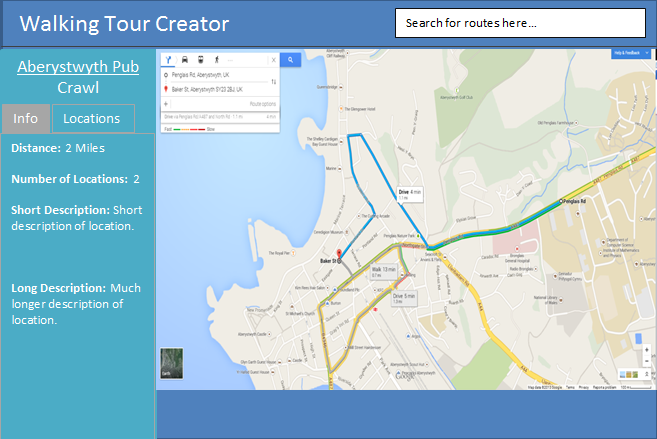
\includegraphics[width=1\linewidth]{WebUI1}
    }
\end{figure}

This is the first page the user will see once they have started up the web application. 
The page contains a search box to search for routes stored in the database, a sidebar 
containing information about the route and it�s locations and a Google Maps representation of the walk.
\bigskip

The search bar will display a drop down menu as the user starts to type giving the user a list of routes 
associated with the value they enter. The user can then select this route which will then populate the sidebar and Google Map. 
The sidebar will allow the user to toggle between information about the walk and information about the locations, as there is not enough space to contain both.
\clearpage

\section{Gantt chart}
\textbf{Authors: Josh Tumath, Lars H Lunde and Theo Taylor}

\begin{figure}[H]
    \makebox[\linewidth]{
        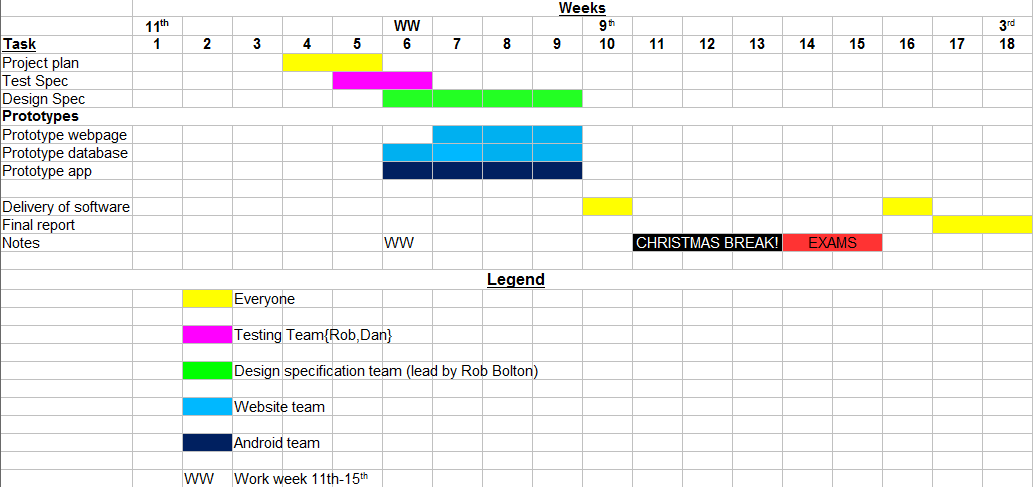
\includegraphics[angle=90,width=0.69\linewidth]{GanttChart}
    }
\end{figure}

\clearpage
The Gantt chart describes the main tasks to be achieved, when each task will start and end, 
which individual or team will carry out each task and the dependencies between different tasks. 
It should contain only major milestones and so should fit on one side of A4 with legible text.

\section{Risk analysis}
\textbf{Authors: James B}
\bigskip

Highlight any parts of the plan which could prove problematic and how the impact of these problems will be mitigated. 
Problems can include slippage due to specific parts taking longer than expected to complete, illness of key group members, 
technical difficulties with systems or complex algorithms and usability issues related to the user interface e.g. \newline
\textit{"A confirmation dialog is essential in step 5 because file deletion is a non-reversible operation"} \newline 
or \newline
\textit{"when the user drags to a part of the map that has not yet been downloaded the area is displayed in grey and the activity indicator is switched on.
 This is essential to avoid confusion with blank areas of the map".} \newline
 
\subsection{Gold plating}
As programmers we sometimes like to show off our skills by adding unnecessary features to our program.
The schema clearly states that there are no extra marks for extra features and so doing this would just
be a waste of programming hours. This can be avoided by having a clear plan of what is needed for the
program before the actual programming starts.

\subsection{Illnesses}
This is an unavoidable risk. It is inevitable that members of the group will fall ill at some point during the year. 
To stop this becoming a problem, any members that fall ill will need to let the group know as soon a possible, so that 
other members can help out with any work that the ill member had been assigned. It is then the responsibility of the 
ill member of the group to then put in some extra work time when he recovers from illness.

\subsection{Time management}
One of the biggest risks for the group is that we will run out of time and that the project will be unfinished in the due date,
or that all members of the group will have to start putting in crazy hours, in a desperate attempt to get the program done.
Again this can be avoided by having a clear plan, where each specific part of the website and program have a clear completion deadline.
 
\subsection{Compromising on design}
In order to get stuck into the harder tasks of a program earlier, programmers will compromise on design on the easier parts of the program,
in order to get stuck into the harder parts. This is also a waste of programming hours as design is arguably the most important part of a program.
 
\subsection{Backups}
The worst situation that could happen is that all the data that the group has been working on gets lost. This is avoided by having multiple backups of our program,
and not just on the same hard drive. These backups need to be made in a separate physical location, and also need to be made every time work has been done on the project.

\subsection{Released project has low quality}
There is always the risk that the project, when completed is of low quality. 
This can be avoided by assuring that everyone is happy with suggested Interface design and everyone is clear on what needs to be done. 
We will also need to ensure a disciplined development is used.

\subsection{Conflicting Ideas}
As programmers, we are all likely to have our own ideas on how we think the app should be developed. 
To avoid any conflict, any issues that an individual may have with the design of the app, 
will have to bring them forward sooner rather than later. This will overall make for a happy group who will be able to work efficiently as a team.

\clearpage
\section{Change Log}
\begin{flushleft}
\begin{tabular}{ | p{1cm} | p{1cm} | p{2.5cm} | p{6cm}| p{1.5cm}| }
\hline
Version & CCF No. & Date & Changes made to document & Changed by \\ \hline
1.0 & N/A & 2013-11-08 & Made first version & LHL \\  \hline
\end{tabular}
\end{flushleft}
\end{document}